Le \textbf{hashtable} è un metodo per accedere alla array, il funzionamento è tramite delle chiavi(\textbf{keys}). Questo garantisce al momento della ricerca tempo constante poiché al record(l'informazione) è associata una chiave. Questa ricerca tramite la chiave per trovare il \textbf{record} viene chiamata anche \textbf{Hashing}.
I \textbf{record} vengono ordinati nel array in modo che \textbf{soddisfino il calcolo dei indirizzi}(cosi la ricerca nel array è più semplice). non sono ordinati per frequenza o valore.\newline\newline
\textbf{Terminologie:}
\begin{itemize}
    \item La funzione che mappa le chiavi e l'associa a una posizione nel array si chiami \textbf{\textcolor{blue}{\code{Hash function}}} denotato con \textbf{h}.
    \item  L'array che immagazzina i \textbf{recrod} viene chiamato \textbf{\textcolor{blue}{\code{Hash Table}}} e viene denotata con la parola \textbf{HT}
    \item Una posizione nella \textbf{hash tabele} viene chiamato \textbf{\textcolor{blue}{\code{slot}}}
    \item slot disponibili nella Hash Table viene denotato con \textbf{M}, i slot sono numerati da \textbf{0 a M-1}
    \item La \textbf{\textcolor{blue}{\code{Home}}} è l'indice restituito dalla \textbf{Hash function}.
\end{itemize}
l'obbiettivo per le \textbf{hash} è quello di organizzare le cose in modo che: Per ogni \textbf{K} chiave e una qualsiasi funzione \textbf{h} abbiamo che  $i =$ \textbf{h($K$)} dove $i$ è l'indice del array dove è immagazzinata l'informazione(\textbf{lo slot dove risiede il record}) della chiave \textbf{K}. la funzione \textbf{h} restituisce un valore tra $0 <= h(K) < M$. L'Obbiettivo è avere che \textbf{HT[i]} contiene il record della chiave \textbf{K}

\subsection{Debolezze generali}
\begin{itemize}
    \item Le \textbf{hashTable} non sono molto utili quando ci sono più \textbf{record} con la stessa chiave (quando permesso);
    \item \textbf{hashTable} non è molto efficiente a cercare in un determinato range
    \item non è efficiente a trovare il massimo o il minimo di un valore di una chiave oppure visitare i record in ordine di chiave
\end{itemize}

\subsection{Utilità}
\begin{itemize}
    \item Quando è utile ? quando vogliamo cercare ogni \textbf{record} con un certa chiave \textbf{K}. le hash vengono utilizzate per i database infatti vengono immagazzinate non solo sulla memoria centrale ma anche sulle memorie come hardisk o ssd.
\end{itemize}

\subsection{Osservazioni}
\begin{itemize}
    \item Nel caso ideale avremo un \textbf{hash table} con \textbf{M solt} e avremo delle chiavi \textbf{k} che vanno da \textbf{0 a M-1}. Cosi facendo avremo che con la chiave \textbf{k} nella \textbf{Hashtable} avrò \textbf{HT[k]} che contiene il \textbf{record} a cui è associato la chiave \textbf{k}. nel caso ideale usiamo tutti le chiavi. quindi a ogni chiave è associato un solo elemento.
    
    \item ovviamente questo se L'Intervallo delle possibili chiavi combacia con il numero di \textbf{slot}
    
    \item nel caso reale questo non avviene, se abbiamo che il range di chiavi è tra 0 e 65.535 dovremmo avere come minimo 65.535 slots però se abbiamo un aspettativa di utilizzare solo 1000 chiavi allora avremo altri 64.535 slots che non saranno mai utilizzatati.
    
\end{itemize}

\subsection{Risoluzione}
\begin{itemize}
    \item Quindi dobbiamo creare una funzione hash \textbf{h} che può mappare un grande intervallo di chiavi nel più piccolo numero di \textbf{slot} quindi in un \textbf{hash table} più piccola possibile.
    \item Questo perché di solito ci sono \textbf{sempre più possibili chiavi} che \textbf{slot}
\end{itemize}
\subsubsection{Problema(collisioni)}
\begin{itemize}
    \item Questa soluzione può portare a \textbf{collisioni} perché per due chiavi $K_1$ e $K_2$ po accadere che h($K_1$) $=$ $\beta$ $=$ h($K_2$)  dove $\beta$ è uno \textbf{slot} della \textbf{tabla hash}
    
    \item La ricerca di un record con valore chiave \textbf{K} in un database organizzato mediante\textbf{ hashing} segue una procedura in due passaggi: 
    \begin{itemize}
        \item 1. Calcolare la posizione della tabella \textbf{ h(K)}.
        \item 2. A partire dallo slot \textbf{h(K)}, individuare il \textbf{record} che contiene la \textbf{chiave} \textbf{K} utilizzando (se necessario) un criterio di \textbf{risoluzione delle collisioni}.
        
    \end{itemize}
  
\end{itemize}

\subsection{Funzione di Hash}
\begin{itemize}
    \item Lo scopo della \textbf{funzione Hash} è di utilizzare meno \textbf{slot} possibili per un certo \textbf{intervallo di chiavi}, ovviamente è impossibile evitare le \textbf{collisioni} in questo caso.
    \item in modo probabilistico meno \textbf{slot} abbiamo è più aumenterà la mobilita di \textbf{collisioni} poiché meno spazio disponibile. inoltre al aumentare delle chiavi aumenta di conseguenza la probabilità di \textbf{collisioni}.
    \item  quindi \textbf{diminuire} i slot e \textbf{aumentare} le chiavi aumenta le \textbf{collisioni}
    \item consideriamo, ad esempio, un'aula piena di studenti. Qual è la probabilità che una coppia di studenti condivida lo stesso compleanno (cioè lo stesso giorno dell'anno, non necessariamente lo stesso anno)? Se ci sono 23 studenti, allora le probabilità sono pari che due condivideranno lo stesso compleanno. Questo nonostante il fatto che ci siano 365 giorni in cui gli studenti possono avere compleanni (ignorando gli anni bisestili), nella maggior parte dei quali nessuno studente della classe compie gli anni. Con più studenti, aumenta la probabilità di un compleanno condiviso.
    
\end{itemize}

\textbf{Una funzione Hash si può considerare:}
\begin{itemize}
    \item \textbf{Indifferente:} va bene qualsiasi funzione che prende una
    chiave e restituisce uno slot.
    \item \textbf{Pessimo:} per qualsiasi chiave restituisce lo stesso slot: la
    tabella di hash non ci aiuta nella ricerca.
    \item \textbf{Ottimo:} ogni slot ha la stessa probabilità di venir colpito.
\end{itemize}

\subsection{Distribuzione delle chiavi}
\begin{itemize}  
    \item Per poter controllare la \textbf{distribuzione degli slot} (quante volte viene colpito uno slot o possibilità che un slot possa essere colpito), \textbf{dovremmo conoscere la distribuzione delle chiavi}(la possibilità che una chiave esca).
    \item Di solito conosciamo il range di valori che le chiavi
    possono assumere.
    \item A volte la distribuzione delle chiavi all’interno del range ci è
    favorevole:
    \begin{itemize}
        \item \textbf{Esempio} distribuzione uniforme delle chiavi(il che significa che ogni possibile chiave avrebbe la stessa probabilità di uscire): basta
        dividere il range in parti uguali.
        Questa frase si riferisce a un esempio di distribuzione uniforme delle chiavi all'interno di un certo intervallo di valori.

        Immagina di avere un intervallo di valori interi da \textbf{0 a 1000}
        e di voler distribuire le chiavi all'interno di questo intervallo in modo uniforme. \textbf{Dividere il range} in parti uguali significa che puoi suddividere l'intervallo totale in \textbf{segmenti} di uguale dimensione.
        
        Ad esempio, se vuoi distribuire le chiavi uniformemente su \textbf{10 segmenti o slot} \textbf{(o "parti uguali")}, puoi fare quanto segue:
        \begin{itemize}
            \item \textbf{Segmento 1:} da 0 a 100
            \item \textbf{Segmento 2:} da 101 a 200
            \item \textbf{Segmento 3:} da 201 a 300
            \item \textbf{Segmento 10:} 901 a 1000
        \end{itemize}
        Ogni segmento ha la stessa dimensione (in questo caso, 100) e contiene un decimo dell'intervallo totale di chiavi. Distribuire le chiavi in questo modo assicura che ogni segmento abbia la stessa probabilità di essere selezionato, garantendo così una distribuzione uniforme delle chiavi all'interno dell'intervallo.

    \end{itemize}
    
    \item Purtroppo la fortuna è rara, e in genere le chiavi risultano
    ammucchiate in alcune parti e rare altrove.
    \item In questi casi la scelta della funzione di hash è critica,
    \item ma dovrebbe partire dalla conoscenza della distribuzione
    delle chiavi.
\end{itemize}

\subsubsection{Perché distribuzioni non uniforme}
\textbf{avvolte le cattive distribuzioni non sono solo sfortuna:}
\begin{itemize}
    \item 1. Distribuzione di Zipf (Es: città grosse e piccole).
    \item 2. La raccolta dei dati introduce bias (Es: arrotondamenti dei
    numeri).
    \item 3. La prima lettera delle parole inglesi (e italiane e . . . ) non è
    uniforme.
\end{itemize}
\subsubsection{Esempi di funzioni di Hash}
\begin{tcolorbox}[width=15cm, boxsep=10pt]
    \textbf{16 slots:}
    \lstinputlisting{Capitoli/HashTable/Esempi/Es1HasFun.txt} 
    \begin{itemize}
        \item Lo slot dipende solo dai quattro bit meno significativi, che
        possono avere una cattiva distribuzione.
        \item Esempio di una scelta tipica: \%M: la scelta della
        dimensione della tabella di hash ha spesso un effetto
        importante sulle prestazioni.
    \end{itemize}
\end{tcolorbox}
\newpage
\textbf{Un altro esempio:}
\begin{itemize}
     \item Metodo mid-square:
    \item Fai il quadrato della chiave.
    \item Prendi gli $r$ bit centrali.
    \item Ottieni uno slot in $\left[0, 2^r - 1\right]$.
    \item Esempio:
    \begin{itemize}
        \item Chiavi: numeri decimali di 4 cifre.
        \item $M = 100$ (2 cifre decimali $\Rightarrow r = 2$)
        \item \textbf{Chiave}: 4567, al quadrato: 208\textbf{57}489
        \item Tutte le cifre contribuiscono a \textbf{57} quindi ci sarà più varianza e meno probabilità che esca lo stesso numero
    \end{itemize}
    \begin{center}
        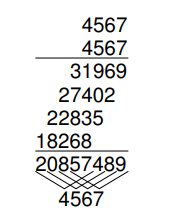
\includegraphics[scale = 0.8]{Capitoli/HashTable/Esempi/moltipilicazione.png}
    \end{center}

\newpage
    \subsection{Gestione delle collisioni}
    \item In pratica, le \textbf{collisioni} non possono venir escluse a priori,
    quindi vanno gestite.
    \item  Due classi principali, con:
    \begin{itemize}    
        \item \textbf{Hashing Aperto}(o con catene separate): le collisioni vengono immagazzinate fuori della tabella di   \textbf{hash}.
        \item  \textbf{Hashing Chiuso} : dentro la tabella di hash, in un altro slot
    \end{itemize}
    
\subsection{Open Hashing (indirizzamento chiuso)}
Nel \textbf{\textcolor{blue}{\code{Open Hashing}}} per ogni \textbf{slot} avremo un \textbf{record} , nel caso in cui ci fosse una \textbf{collisione} si creerebbe una lista \textbf{linkata}. in uno \textbf{slot} potremmo avere più \textbf{record} \textbf{linkati} fra di loro. \newline\newline
\textbf{Benefici:}
\begin{itemize}
    \item Questo metodo è molto semplice da gestire, di solito si può ordinare gli elementi della linked list tramite dei criteri, del tipo:
    \begin{itemize}
        \item Per numero di accessi
        \item Per ordine dei chiave
        \item a caso
    \end{itemize}
    \item  ovviamente dare un ordinamento può ritornare utile poiché il \textbf{tempo medio potrebbe beneficiarne}. se esempio accedo molto spesso alla chiave \textbf{"cane"} mediamente il mio $\theta$ medio sarà migliore.
\end{itemize}
    \begin{center}
        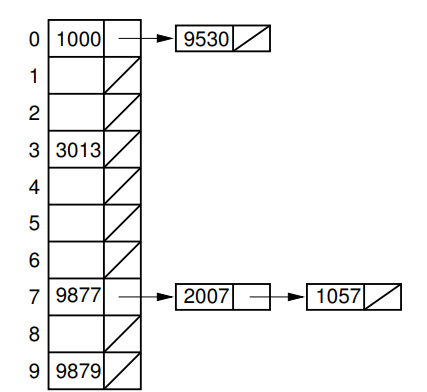
\includegraphics[scale = 0.6]{Capitoli/HashTable/Esempi/OpenHashing.png}
    \end{center}
\end{itemize}
\newpage
Se abbiamo \textbf{M} slot e \textbf{N} record da immagazzinare avremo che in ogni slot ci sarà $N \div M$. se invece stiamo nel caso in cui abbiamo \textbf{più slot} che \textbf{record} si spera che avremo \textbf{meno slot} possibili \textbf{con più di un record.} \newline
se ogni slot ha solo un record il tempo medio di accesso è $\theta(1)$.\newline\newline
\textbf{Svantaggi:}
\begin{itemize}
    \item La \textbf{linked list} o comunque delle strutture che hanno dei salti da un blocco al altro della memoria sono efficienti solo nella memoria primaria
    \item Nella \textbf{memoria secondaria} sarebbe poco efficiente poiché dobbiamo \textbf{accedere} più volte alla \textbf{memoria secondaria}(Sappiamo che la memoria secondaria è molto più lenta).
\end{itemize}
\subsection{Closed Hashing (indirizzamento aperto) Con Buckets}
\textbf{\textcolor{blue}{\code{{L'Hashing chiuso}}}} utilizza i \textbf{Buckets} quindi per\textbf{ M} slot e \textbf{B} buckets avrò che ogni \textbf{Bucket} avrà $M \div B$ slots. \newline
Ogni volta che la \textbf{Hash function} darà un indice questo sarà il numero del \textbf{bucket}. nel momento del inserimento del record dovrò partire dal inizio del \textbf{bucket} e scorrere finché non trovo uno slot libero. se il \textbf{bucket} è pieno il record sarà inserito in un \textbf{overflow bucket} che ha spazio "infinito"
\begin{center}
    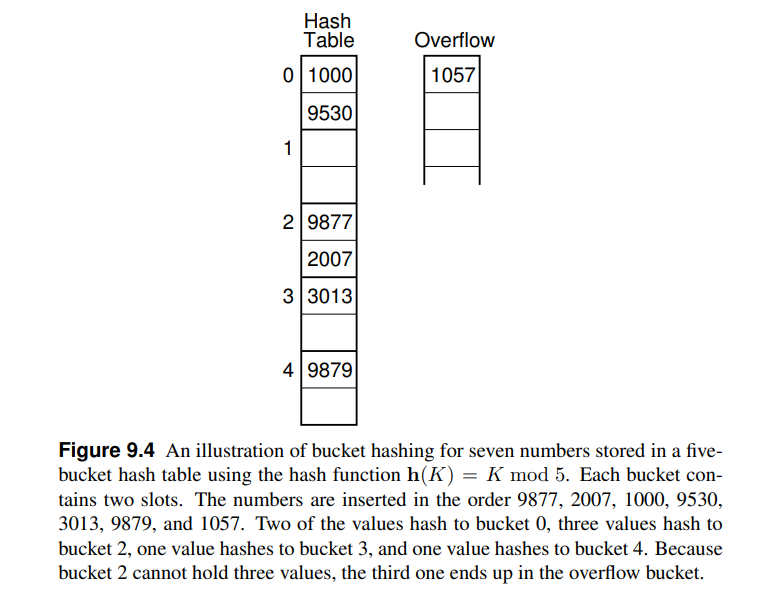
\includegraphics[scale = 0.6]{Capitoli/HashTable/Esempi/ClosingHash.png}
\end{center}
Una \textbf{buona} implementazione della \textbf{Hash function} e riempire sempre tutti i \textbf{bucket} e cercare di andare meno possibile nel \textbf{overflow bucket}

\subsubsection{Ricerca dei record}
Quando dobbiamo ricercare i record nel \textbf{HashTable} dobbiamo utilizzare la La \textbf{Hash Function} con la chiave \textbf{K} per determinare il \textbf{bucket}. Possiamo ricadere in vari casi:
\begin{itemize}
    \item Ricercare il \textbf{Bucket} dove risiede il \textbf{record} associato alla \textbf{chiave K}(la Chieve \textbf{K} ci serve a trovare il \textbf{bucket} tramite la \textbf{funzione di hash}, ma \textbf{K} ci servirà a trovare il corretto \textbf{record} nel \textbf{bucket}). Successivamente aver trovato il \textbf{bucket} si ricercherà il \textbf{record} con la chiave \textbf{K} nel \textbf{bucket}. Se \textbf{ricercando} troviamo una posizione vuota e non abbiamo ancora trovato il \textbf{record} allora quest'ultimo non è presente.
    
    \item Se ricercando  finisce il \textbf{bucket} dovremo andare in quello di \textbf{overflow}. per determinare se il \textbf{record} c'è oppure no dobbiamo navigare tutto il \textbf{bucket di overflow}
\end{itemize}

\subsubsection{Problemi e variante del bucket}
Il problema principale è che iniziando sempre a inserire dal primo elemento del \textbf{bucket} c'è più probabilità di \textbf{collisione} , di conseguenza più accessi da fare. Quindi accedo al primo slot se c'è \textbf{collisione} scendo al secondo slot , controllo il secondo slot se c'è \textbf{collisione} vado avanti ... e cosi via.\newline
\textbf{La variante}:
\begin{itemize}
    \item Quando inserisco un \textbf{record} accederò a uno \textbf{slot} \textbf{casuale} del \textbf{bucket} cosi diminuendo la probabilità di \textbf{collisione}
    \item Poi scorro finché non trovo una posizione libera, se arrivo alla fine del \textbf{bucket} risalgo al inizio e continuo , questa ricerca di inserimento finirà quando torno al punto di partenza.
    \item il \textbf{bucket} quindi è "circolare"
\end{itemize}
\begin{center}
    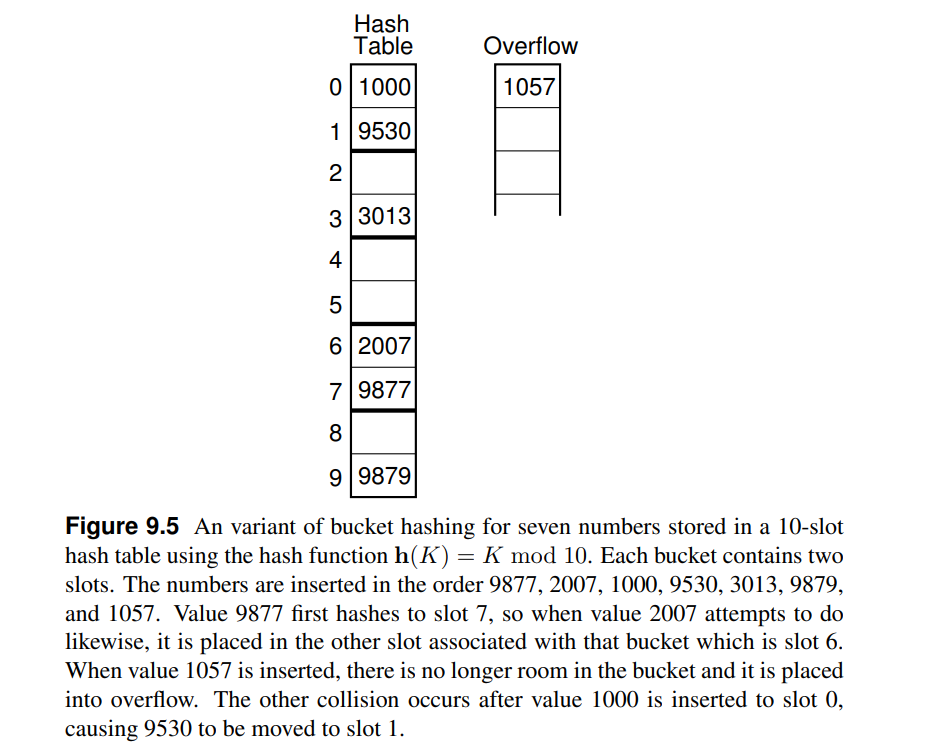
\includegraphics[scale = 0.6]{Capitoli/HashTable/Esempi/VarianteBuckets.png}
\end{center}
\newpage
\subsection{Closed Hashing (indirizzamento aperto) Con Linear Probing}
Questo metodo non ha i \textbf{bucket}. 
\subsubsection{Inserimento:}
Quando andiamo alla \textbf{Home} e accade una collisione durante l'inserimento si andrà a cercare nello slot successivo della \textbf{home}, se c'è uno \textbf{slot} libero si inserisce altrimenti si va avanti. Quindi \textbf{l'inserimento} cercherà dalla \textbf{home} in poi uno slot libero dove inserire l'elemento(La HashTable è circolare).\newline\newline
\textbf{Passaggi}:
\begin{itemize}
    \item Primo passo ottenere la \textbf{Home} con la funzione di \textbf{Hash}.
    \item Partendo dalla \textbf{home} trovare uno slot libero (\code{EMPTYKEY}) per ottenere \textbf{l'offeset} da aggiungere alla \textbf{home} si richiama la \textbf{probe function}( \textbf{P}$(K, i) = i$ dove $i$ è \textbf{L'offset})
    \item l'inserimento non parte propino se non ho almeno due slot liberi , questo perché lo slot libero ci servirà nella ricerca.
\end{itemize}
\begin{tcolorbox}[width=15cm, boxsep=10pt]
     \textbf{Inserimento}
    \lstinputlisting{Capitoli/HashTable/Esempi/InserimentoProping.txt} 
\end{tcolorbox}
La sequenza di slot dalla \textbf{Home} in poi viene chiamata  \textbf{\textcolor{blue}{\code{probe sequence}}} la funzione che restituisce \textbf{l'offset} da aggiungere alla \textbf{Home} è chiamata \textbf{\textcolor{blue}{\code{probe Function}}}
\newpage
\subsubsection{Ricerca}
Se si segue la \textbf{\textcolor{blue}{\code{probe sequence}}} la fase di ricerca è possibile. questo perché se nel inserimento non si  segue il \textbf{probe sequence} non abbiamo la sicurezza che se incontro uno spazio vuoto sono sicuro che la chiave \textbf{K} non c'è nella hash.\newline\newline
\textbf{Passaggi}:
\begin{itemize}
    \item Trovo la \textbf{Home} con la funzione di \textbf{Hash}
    \item Se la \textbf{home} non contiene \textbf{K} vado al successivo, quindi utilizzando la \textbf{probe Function} calcolo offset è vado avanti.
    \item mi fermerò quando lo trovo oppure quando trovo uno slot vuoto, questo indicherà che non c'è l'emento con chiave \textbf{K}
\end{itemize}
\begin{tcolorbox}[width=16cm, boxsep=10pt]
     \textbf{Ricerca}
    \lstinputlisting{Capitoli/HashTable/Esempi/RicercaProping.txt} 
\end{tcolorbox}
\newpage
\subsubsection{Primary Clustering}
Il \textbf{Proping primario} è il peggior metodo per risolvere le \textbf{collisioni}, perché soffre del \textbf{Primary Clustering}. Questo problema tende a far raggruppare due insieme di record. 
\begin{center}
    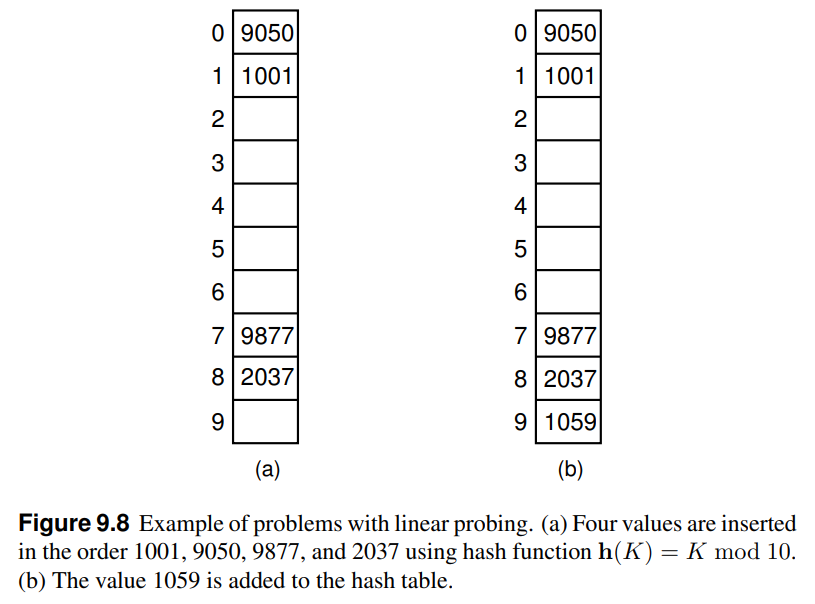
\includegraphics[scale = 0.36]{Capitoli/HashTable/Esempi/ClusteringPrimario.png}
\end{center}
Come notiamo nella figura sopra i due blocchi  si  tendono ad unirsi poiché le probabilità che il prossimo record sia inserito nella posizione \textbf{2} è del \textbf{0.6} quindi $6/10$ invece per tutti i \textbf{slot} da \textbf{3 a 6} è una possibilità su \textbf{10 quindi 0.1} \newline
questo perché se colpisco \textbf{7,8,9,0 o 1} andranno tutti a inserire nello \textbf{slot 2} poiché L'Inserimento andrà avanti finché non trova uno slot vuoto. 
\begin{enumerate}
    \item \textbf{Aumento del Tempo di Ricerca:}

    Quando si verifica clustering primario, le operazioni di ricerca richiedono più tempo perché più elementi devono essere esaminati. Se molte chiavi si trovano nello stesso cluster, bisogna scorrere una lunga sequenza di celle per trovare l'elemento desiderato.

    \item \textbf{Riduzione delle Prestazioni di Inserimento e Cancellazione:}

    Le operazioni di inserimento e cancellazione diventano meno efficienti perché richiedono il trattamento di collisioni. In presenza di un grande cluster, un nuovo elemento che collide con questo cluster deve essere inserito alla fine del cluster, aumentando così la lunghezza della sequenza.
    
    \item \textbf{Degradazione dell'Equilibrio della Tabella Hash:}

    L'accumulo di elementi in poche aree della tabella riduce l'efficacia della funzione di hash nel distribuire uniformemente le chiavi. Questo porta a un uso inefficiente dello spazio della tabella hash e può richiedere ridimensionamenti più frequenti.
    
    \item \textbf{Effetto Cascata:}

    Una volta che si forma un cluster, è probabile che questo cluster cresca più velocemente di altre aree della tabella, poiché le collisioni successive tenderanno ad aggregarsi ulteriormente al cluster esistente.
\end{enumerate}

\subsection{Miglioramento gestione collisioni (Hashing chiuso)}
Ci sono vari modi per risolvere il  \textbf{primary clustering}, il metodo più veloce è quello di aggiungere una costante moltiplicativa al \textbf{offset}.\newline
\begin{tcolorbox}
    \begin{itemize}
        \item Quindi la \textbf{\textcolor{blue}{\code{funzione di Proping}}} diventa nel seguente modo \textbf{P($K,i$)} $= ci$ dove \textbf{c} è la costante moltiplicativa.
        \item La \textbf{\textcolor{blue}{\code{probe sequence}}} sarà del tipo \textbf{(h($K$)$ + ic$) mod $M$}. il modulo di M per far in modo che il numero sia sempre al interno del numero di slot.
    \end{itemize}
\end{tcolorbox}
Un buona \textbf{\textcolor{blue}{\code{probe sequence}}} dovrebbe fare in modo che tutti i slot vengano visionati prima di ritornare alla \textbf{home}. Sfortunatamente in questo caso non è cosi.\newpage
\textbf{Esempio}
\begin{itemize}
    \item Se ho $c = 2$ , la home position  è pari e Il numero di slot M è pari allora avrò che capiterò sempre e solo sui slot pari, al contrario se la home position dispari andrò solo i quelli dispari.
    \item quindi non andrò mai a visionare tutti i slot ma solo una parte.
\end{itemize}
Essendo \textbf{M} variabile potrei avere dei problemi. Osserviamo che abbiamo \textbf{due blocchi}: il blocco dei  \textbf{numeri pari} e quello dei \textbf{numeri dispari}. Se uno dei due si riempisse troppo e l'altro rimarrebbe mezzo vuoto avremo che da una parte le\textbf{ prestazioni sono ottime} dal altro \textbf{pessime}. Questo non ci piace perché va a impattare in modo\textbf{ negativo} mediamente su tutta la struttura. Detto in poche parole il gioco non vale la candela!
\subsubsection{Risoluzione:}
Per risolvere questo problema basterà prendere una \textbf{c} che non abbia divisori in comune con la \textbf{M}(oppure prendere M primo) cosi facendo si prenderanno tutti i \textbf{solt}. Quindi se ho $M = 10$ , \textbf{c} dovrà essere \textbf{1,3,7} oppure \textbf{9}. Se invece $M = 11$ basterà un numero \textbf{tra 0 e 10}. Osserviamo che questo però non ci salverà dal \textbf{clustering primario} poiché con \textbf{c = 2} le chiavi $k_1$ e $k_2$ potrebbero avere una \textbf{\textcolor{blue}{\code{probe sequence}}} che converge nella stessa. Se \textbf{h($k_1$) = 3} la sequenza è \textbf{3,5,7,9} e cosi via. Se \textbf{h($k_2$) = 5} la sequenza è \textbf{5,7,9} e cosi via. come possiamo vedere dopo un certo punto è la stessa \textbf{\textcolor{blue}{\code{probe sequence}}}. in sintesi questo metodo non risolve il \textbf{clustering primario}

\subsubsection{Risoluzione Definitiva Clustering Primario}
Esistono due modi per risolvere \textbf{Clustering Primario} il primo  è avere un \textbf{offset} casuale , cosi facendo è statisticamente improbabile che due chiavi hanno la stessa \textbf{\textcolor{blue}{\code{probe sequence}}}. Questo è impossibile poiché  se avessimo un offset casuale non potremmo più ricercare un record poiché per una stessa chiave abbiamo un offset sempre diverso. Quindi posiamo usare dei numeri \textbf{pseudo-casuali}, questa tecnica viene chiamata \textbf{\textcolor{blue}{\code{pseudo-random probing}}}\newline\newline
\textbf{Funzionamento}:
\begin{itemize}
    \item Avremo quindi che \textbf{(h($K$) + $r_i$) mod $M$} sarà lo slot del inderimento/ricerca
    \item $r_i$ è il valore nella \textbf{i-esima} cella del vettore che conterrà valori casuali ma fissi, cioè dopo aver deciso i numeri casuali quest'ultimi non cambieranno. non sono valori casuali ma permutazioni dei valori da 1 a M-1.
    \item \textbf{\textcolor{blue}{\code{probe Function}}} è \textbf{p($K,i$) $=$ \code{Perm[$i-1$]}} dove \textbf{\code{Perm}} è un array di lunghezza \textbf{M-1} contando la \textbf{permutazione casuale} dei valori fa \textbf{ 1 a M-1}.
    \textbf{Quindi per chiavi diverse non avrò mai la stessa sequenza di probing.}
\end{itemize}
\begin{center}
    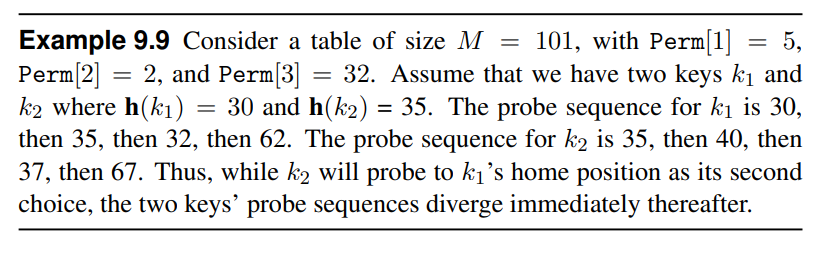
\includegraphics[scale = 0.6]{Capitoli/HashTable/Esempi/EsempioPseudo.png}
\end{center}
Il secondo metodo per risolvere il \textbf{clustering primario} è \textbf{\textcolor{blue}{quadratic probing}} dove la \textbf{funzione di proping} è \textbf{p($K,i$) $=$ $c_1 i^2 + c_2i + c_3$}. \newline
il caso più facile di è\textbf{ p($K,i$) = $i^2$} quindi \textbf{(h($K$) + $i^2$) mod $M$}
\begin{center}
    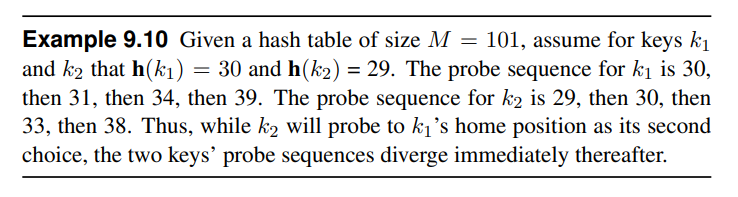
\includegraphics[scale = 0.6]{Capitoli/HashTable/Esempi/EsempioQuadratic.png}
\end{center}
il problema del \textbf{clustring quadratico} è che alcuni slot non verranno mai visionati, se per esempio avessimo una \textbf{hashtable} di \textbf{size 3} quindi abbiamo i slot \textbf{0,1 e 2} possiamo dire con certezza che \textbf{2} non sarà mai \textbf{visionato}. 
un modo semplice di risolvere è di avere \textbf{M} come numero primo cosi sicuramente meta tabella potrà essere riempita. oppure usare una \textbf{funzione di proping} del tipo \textbf{p($K,i$) $=$($i^2 + i$)/$2$} e M = $2^S$(M come potenza di 2) cosi facendo ogni \textbf{slot} sarà riempito.

\subsubsection{Clustering Secondario}
Il \textbf{\textcolor{blue}{\code{secondary clustering}}} si genera con le due nuove \textbf{funzione di proping}. Il \textbf{\textcolor{blue}{\code{secondary clustering}}} non genera dei cluster contigui ma delle \textbf{chiavi diverse} \textbf{K} possono avere la stessa \textbf{\textcolor{blue}{\code{probe sequence}}} e cosi facendo avendo dei cluster, però non contigui.
\begin{center}
    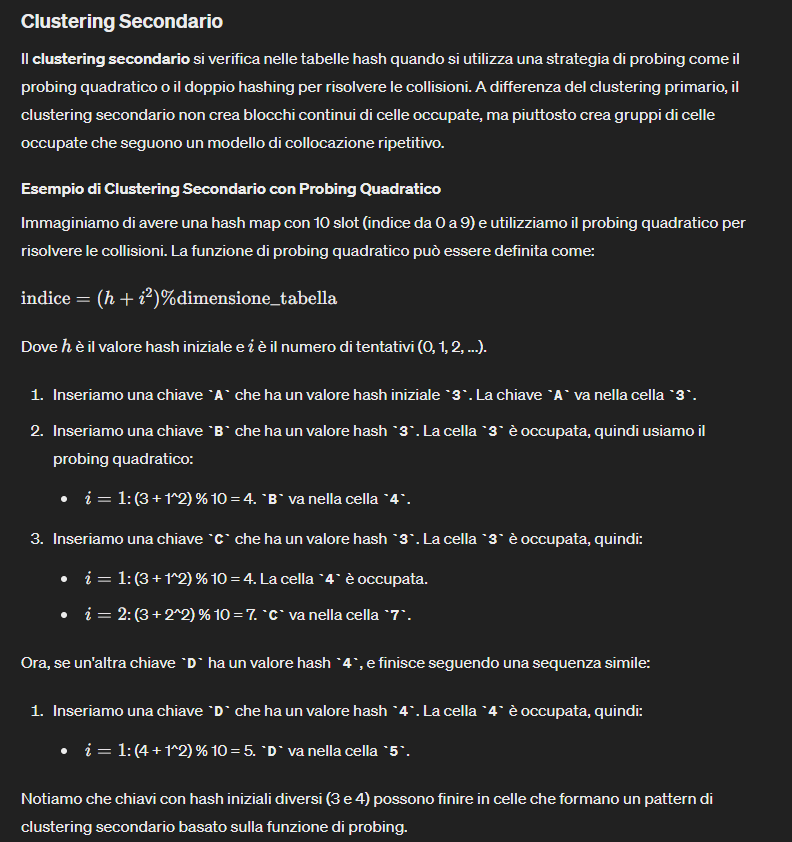
\includegraphics[scale = 0.8]{Capitoli/HashTable/Esempi/Esempio clustering.png}
\end{center}
\newpage
\subsection{Risoluzione Clustering Secondario}
Per risolvere il\textbf{ clustering secondario} si utilizza una \textbf{seconda funzione hashing} , il risultato di questa seconda funzione viene usata come \textbf{costante moltiplicativa}. quindi avremo \textbf{p($K,i$) $=$($i * h_2(K)$)}. questa $h_2$ restituisce un valore tra $1 <= h_2 <= M-1$
\begin{center}
    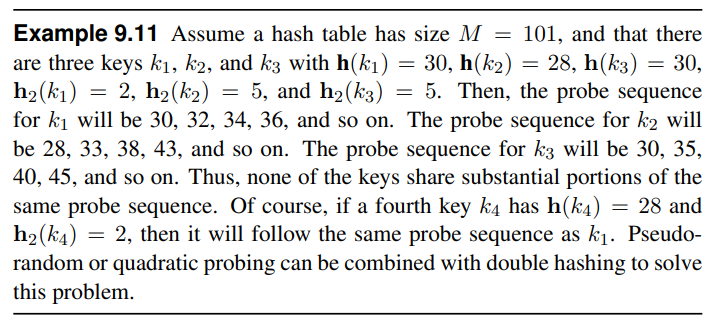
\includegraphics[scale = 0.6]{Capitoli/HashTable/Esempi/DoppioHashing.png}
\end{center}
questo ci garantisce di non avere \textbf{\textcolor{blue}{\code{probe sequence}}} uguali per chiavi diverse

\subsection{Risoluzione problema cancellazione}
La cancellazione deve affrontare due problemi:
\begin{itemize}
    \item \textbf{Cancellare un record} potrebbe creare dei problemi nella ricerca. Quando noi inseriamo un dato seguiamo una sequenza di \textbf{probing}, nel momento in cui \textbf{cancelliamo} un elemento potremmo rompere questa sequenza. Questo significa che nel inserimento siamo passati per un elemento che ora nella ricerca non c'è più(poiché cancellato) quindi troveremo uno \textbf{slot vuoto} prima del dovuto, cosi facendo non visiteremo tutta la sequenza di \textbf{probing}.
    \item  Il secondo problema che dobbiamo far in modo che lo slot che vogliamo cancellare sia riutilizzabile anche dopo la cancellazione 
\end{itemize}
\textbf{La risoluzione è molto semplice:} utilizzeremo delle \textbf{tombstone}(pietre tomabali). metteremo una \textbf{TombStone} quando cancelliamo, che sarà valutato come uno \textbf{slot pieno}nella ricerca, come \textbf{slot vuoto} nel inserimento. Quindi nel inserimento se \textbf{troviamo} una \textbf{tombstone} inseriamo, invece nella ricerca continuiamo.
\newpage

\subsection{Considerazioni}
Quindi quando si fa un \textbf{HashMap} si deve guardare:
\begin{itemize}
    \item Un ottima distribuzione dei slot quindi avere meno collisioni possibili
    \item una buona cosa di solito quando si vuole una ottima distribuzione è usare i \textbf{numeri primi}, poiché i \textbf{numeri primi} non hanno divisori in comune con nessuno. quindi i numeri che hanno gli stessi fattori produrranno valori \textbf{hash} con \textbf{pattern ripetitivi}. Usando un \textbf{numero primo}, si \textbf{riduce} questa ripetizione. questo perché si farà $h_1$(k) \% \textbf{M}
    \item  diciamo che per una distribuzione non uniforme delle chiavi dovrebbe ridurre il numero di collisioni
    \item ricordiamo che le chiavi nel caso reale non hanno una distribuzione uniforme.
\end{itemize}